\documentclass[aspectratio=169,11pt]{beamer}

\usepackage[utf8]{inputenc}
\usepackage[T1]{fontenc}
\usepackage[spanish]{babel}
\usepackage{lmodern}
\usepackage{graphicx}
\usepackage{booktabs}
\usepackage{array}
\usepackage{tikz}
\usepackage{amsmath}
\usetikzlibrary{arrows.meta,positioning,calc}

% --- Estilo moderno con mayor presencia visual ---
\usetheme{default}
\useinnertheme{circles}
\usefonttheme{professionalfonts}
\usefonttheme{structurebold}
\renewcommand{\familydefault}{\sfdefault}

\definecolor{Primary}{HTML}{0B1220}    % texto principal (azul noche)
\definecolor{Accent}{HTML}{0284C7}     % acento principal (azul)
\definecolor{AccentAlt}{HTML}{0F766E}  % acento secundario (teal profundo)
\definecolor{AccentSoft}{HTML}{E0F2FE} % azul suave
\definecolor{SoftBG}{HTML}{F8FAFC}     % fondo suave
\definecolor{Warm}{HTML}{F59E0B}       % acento cálido
\definecolor{Line}{HTML}{CBD5E1}       % líneas sutiles

\setbeamercolor{normal text}{fg=Primary,bg=white}
\setbeamercolor{structure}{fg=Accent}
\setbeamercolor{frametitle}{fg=Primary,bg=SoftBG}
\setbeamercolor{title}{fg=Primary}
\setbeamercolor{subtitle}{fg=Accent!90!Primary}
\setbeamercolor{author}{fg=Primary}
\setbeamercolor{institute}{fg=Primary!75!black}
\setbeamercolor{date}{fg=Primary!65!black}
\setbeamercolor{item}{fg=Accent}
\setbeamercolor{enumerate item}{fg=Accent}
\setbeamercolor{footline}{fg=Primary!60!white,bg=white}
\setbeamercolor{block title}{fg=white,bg=Accent}
\setbeamercolor{block body}{fg=Primary,bg=AccentSoft!35!white}

\setbeamerfont{title}{size=\LARGE,series=\bfseries}
\setbeamerfont{subtitle}{size=\large}
\setbeamerfont{frametitle}{size=\Large,series=\bfseries}
\setbeamerfont{author}{size=\normalsize}
\setbeamerfont{institute}{size=\small}
\setbeamerfont{date}{size=\small}
\setbeamerfont{footline}{size=\tiny}

\setbeamertemplate{navigation symbols}{}
\setbeamertemplate{caption}[numbered]
\setbeamertemplate{itemize items}[circle]
\setbeamertemplate{enumerate items}[default]
\setbeamertemplate{blocks}[rounded][shadow=false]
\setbeamersize{text margin left=0.85cm,text margin right=0.85cm}

% Fondo con acentos geométricos
\setbeamertemplate{background}{%
  \begin{tikzpicture}
    \useasboundingbox (0,0) rectangle (\the\paperwidth,\the\paperheight);
    \ifnum\theframenumber=1
      \fill[Accent!8] (0,0) rectangle (\paperwidth,0.34\paperheight);
      \fill[Primary] (0,0) rectangle (0.42cm,\paperheight);
      \fill[Accent!10] (\paperwidth-3.6cm,\paperheight-3.0cm) circle (2.8cm);
      \fill[AccentAlt!10] (\paperwidth-1.4cm,0.9cm) circle (1.7cm);
    \else
      \fill[Accent!5] (\paperwidth-1.7cm,-0.5cm) circle (2.1cm);
      \fill[AccentAlt!5] (-0.7cm,\paperheight-0.9cm) circle (1.7cm);
      \fill[Line!45] (0,\paperheight-0.06cm) rectangle (\paperwidth,\paperheight);
    \fi
  \end{tikzpicture}%
}

% Frametitle destacado
\setbeamertemplate{frametitle}{%
  \nointerlineskip
  \begin{beamercolorbox}[wd=\paperwidth,ht=4.2ex,dp=1.8ex,leftskip=0.85cm,rightskip=0.85cm]{frametitle}
    {\color{Accent}\vrule width 0.28em height 2.2ex\hspace{0.55em}}%
    \usebeamerfont{frametitle}\insertframetitle
  \end{beamercolorbox}%
  \nointerlineskip
  {\color{Accent!70}\hspace*{0.85cm}\rule{\dimexpr\paperwidth-1.7cm\relax}{0.6pt}}%
  \vspace{0.25em}%
}

% Pie de página con barra de progreso
\setbeamertemplate{footline}{%
  \leavevmode%
  \begin{tikzpicture}
    \useasboundingbox (0,0) rectangle (\paperwidth,0.5cm);
    \fill[Line!55] (0,0.42cm) rectangle (\paperwidth,0.5cm);
    \ifnum\inserttotalframenumber>0
      \pgfmathsetmacro{\progress}{\insertframenumber/\inserttotalframenumber}
    \else
      \pgfmathsetmacro{\progress}{0}
    \fi
    \fill[Accent] (0,0.42cm) rectangle ({\progress*\paperwidth},0.5cm);
    \node[anchor=west, font=\tiny, text=Primary!70!black] at (0.85cm,0.18cm) {\insertshorttitle};
    \node[anchor=east, font=\tiny, text=Primary!70!black] at (\paperwidth-0.85cm,0.18cm) {\insertframenumber{} / \inserttotalframenumber};
  \end{tikzpicture}%
}

% Portada con mayor presencia visual (slide 1 del guion)
\setbeamertemplate{title page}{%
  \vspace*{0.3cm}
  \hspace*{0.35cm}%
  \begin{minipage}{0.75\paperwidth}
    {\color{Accent}\rule{1.8cm}{0.22cm}\par}
    \vspace{0.45em}
    {\usebeamerfont{title}\usebeamercolor[fg]{title}\inserttitle\par}
    \vspace{0.35em}
    {\usebeamerfont{subtitle}\usebeamercolor[fg]{subtitle}\insertsubtitle\par}
    \vspace{0.7em}
    {\color{Line}\rule{\linewidth}{0.6pt}\par}
    \vspace{0.5em}
    {\usebeamerfont{author}\insertauthor\par}
    \vspace{0.35em}
    {\usebeamerfont{institute}\usebeamercolor[fg]{institute}\insertinstitute\par}
    \vspace{0.55em}
    {\usebeamerfont{date}\usebeamercolor[fg]{date}\insertdate\par}
  \end{minipage}\hfill
  \vfill
}

\graphicspath{{../informe/}}

\title[Retratos profesionales controlados]{Retratos profesionales con IA, decididos por el usuario}
\subtitle{Sistema generativo interactivo con feedback humano y agente explicador}
\author[Gálvez \and Meneses \and Ore]{Grupo 7: José Guillermo Gálvez Pacori \and Matías Alonso Meneses Roncal \and Alejandro Joel Ore García}
\institute[UTEC]{CS5363 Planificación y Toma de Decisiones en IA · UTEC 2026-2\\
Docentes: Dra. Aurea Soriano-Vargas; Mg. Robert Junior Buleje Del Carpio}
\date{2026}

\begin{document}

%------------------------------------------------
% 1. Portada
\begin{frame}
  \titlepage
\end{frame}

%------------------------------------------------
% 2. Problema
\begin{frame}{Un retrato profesional sigue siendo caro o poco fiable}
  \begin{columns}[T]
    \begin{column}{0.6\textwidth}
      \textbf{Problema}
      \begin{itemize}
        \item Una foto profesional de estudio cuesta entre \textbf{50 y 150 USD}, sin contar traslados ni postproducción.
        \item Para un estudiante, es un gasto difícil de asumir.
      \end{itemize}
      \vspace{0.4em}
      \textbf{Alternativa obvia: generadores de imágenes}
      \begin{itemize}
        \item \textbf{Identidad:} el resultado puede no parecerse a la persona.
        \item \textbf{Contexto:} no distinguen LinkedIn, WhatsApp corporativo o GitHub.
        \item \textbf{Transparencia:} el usuario no sabe por qué se propone cada opción.
      \end{itemize}
    \end{column}
    \begin{column}{0.4\textwidth}
      \begin{block}{Nuestra respuesta}
        \begin{itemize}
          \item Generar \textbf{5 variaciones} por foto.
          \item Dejar que la \textbf{persona elija} (aceptar/rechazar).
          \item \textbf{Explicar} sus elecciones con un agente.
        \end{itemize}
      \end{block}
      \vspace{0.4em}
      \centering
      \scriptsize\color{Primary!70} La IA propone; la persona decide.
    \end{column}
  \end{columns}
\end{frame}

%------------------------------------------------
% 3. Design Thinking
\begin{frame}{Design Thinking: del reto a la propuesta de valor}
  \textbf{Pregunta guía (Semana 13)}
  \begin{block}{Reto}
    \emph{¿Cómo facilitar la generación accesible y controlada de retratos profesionales para estudiantes y jóvenes egresados?}
  \end{block}

  \vspace{0.2em}
  \begin{columns}[T]
    \begin{column}{0.48\textwidth}
      \textbf{Perfil de usuario}
      \begin{itemize}
        \item Estudiante de ciclos avanzados o egresado reciente.
        \item Poco presupuesto.
        \item Teme que la IA le deforme la cara.
        \item Necesita una foto distinta para cada red.
      \end{itemize}
    \end{column}
    \begin{column}{0.48\textwidth}
      \textbf{Propuesta de valor}
      \begin{itemize}
        \item \textbf{Funcional:} adapta el retrato a cada red con presets y prompt libre.
        \item \textbf{Social:} proyecta una imagen creíble ante reclutadores y clientes.
        \item \textbf{Emocional:} la persona siempre tiene la última palabra.
      \end{itemize}
    \end{column}
  \end{columns}
\end{frame}

%------------------------------------------------
% 4. Journey map
%------------------------------------------------
%------------------------------------------------
% 4. Journey map
\begin{frame}{Journey map: el usuario decide en cada paso}
  \centering
  \begin{tikzpicture}[
    node distance=0.22cm and 0.22cm,
    jstep/.style={
      rectangle,
      draw=Accent!45,
      rounded corners=3pt,
      align=center,
      font=\scriptsize,
      text width=2.22cm,
      minimum height=1.35cm,
      inner sep=3pt,
      fill=Accent!7,
      text=Primary
    },
    arrow/.style={
      -{Latex[length=2mm]},
      thick,
      draw=Primary!60
    }
  ]
    \node[jstep] (s1) {\textbf{1. Sube y elige}\\Selfie + paquete de 5 estilos};
    \node[jstep, right=of s1] (s2) {\textbf{2. Ve la guía}\\Recorte de cara y bordes del modelo};
    \node[jstep, right=of s2, fill=Warm!14, draw=Warm!65] (s3) {\textbf{3. Recibe opciones}\\5 variaciones en estado \textbf{Pendiente}};
    \node[jstep, right=of s3] (s4) {\textbf{4. Decide}\\Acepta/rechaza, califica y comenta};
    \node[jstep, right=of s4, fill=AccentAlt!12, draw=AccentAlt!55] (s5) {\textbf{5. Comprende}\\Agente resume aceptadas, rechazadas y por qué};

    \draw[arrow] (s1) -- (s2);
    \draw[arrow] (s2) -- (s3);
    \draw[arrow] (s3) -- (s4);
    \draw[arrow] (s4) -- (s5);
  \end{tikzpicture}

  \vspace{0.8em}
  \begin{block}{Principio clave}
    Nada se da por aceptado hasta que la persona vota: el estado \textbf{Pendiente} preserva el control humano en cada variación.
  \end{block}
\end{frame}

%------------------------------------------------
% 5. Arquitectura
\begin{frame}{Arquitectura: de la foto a la explicación}
  \centering
  \begin{tikzpicture}[
    node distance=0.35cm and 0.55cm,
    box/.style={rectangle, draw=Primary!20, rounded corners=3pt, align=center, font=\scriptsize, text width=3.05cm, minimum height=0.95cm, fill=SoftBG, text=Primary},
    accent/.style={box, draw=Accent!35, fill=Accent!8},
    warm/.style={box, draw=Warm!50, fill=Warm!10},
    success/.style={box, draw=AccentAlt!40, fill=AccentAlt!8},
    arrow/.style={-{Latex[length=2mm]}, thick, draw=Primary!55}
  ]
    \node[box] (in) {1. Entrada\\Foto, paquete de estilos, prompt libre};
    \node[warm, right=of in] (safe) {2. Filtro ético\\Bloquea pedidos inapropiados (antes de GPU)};
    \node[box, right=of safe] (prep) {3. Preproceso\\Detecta cara, recorta 512$\times$512, bordes Canny};
    \node[accent, right=of prep] (gpu) {4. Servidor GPU (Colab, T4)\\FastAPI recibe base64 y genera 5 variaciones};
    \node[success, below=0.65cm of gpu] (ui) {5. Interfaz Streamlit\\Variaciones y decisión humana};
    \node[box, left=of ui] (log) {6. Registro JSON\\Decisiones, imágenes y tiempos};
    \node[accent, left=of log] (agent) {7. Agente explicador\\Resumen y fidelidad contra datos};
    \node[success, left=of agent] (out) {8. Salida\\Aceptadas, rechazadas y explicación};

    \draw[arrow] (in) -- (safe);
    \draw[arrow] (safe) -- (prep);
    \draw[arrow] (prep) -- node[above,font=\tiny,text=Primary!70]{base64} (gpu);
    \draw[arrow] (gpu) -- (ui);
    \draw[arrow] (ui) -- (log);
    \draw[arrow] (log) -- (agent);
    \draw[arrow] (agent) -- (out);
  \end{tikzpicture}

  \vspace{0.4em}
  \small
  \begin{itemize}
    \item 8 etapas: de la foto a la explicación. Interfaz local + GPU remota (túnel Cloudflare).
    \item Si no hay GPU: respaldo local con filtros OpenCV (no generativo, para mantener el flujo).
  \end{itemize}
\end{frame}

%------------------------------------------------
%------------------------------------------------
% 6. Preprocesamiento
\begin{frame}{Preprocesamiento: detectar, recortar y describir}
  \begin{columns}[T]
    \begin{column}{0.55\textwidth}
      \small
      \textbf{Pipeline}
      \begin{enumerate}
        \item Detección facial con \textbf{2 clasificadores Haar} (OpenCV).
        \item Recorte \textbf{cuadrado de 512$\times$512 px} centrado en la cara.
        \item Extracción de bordes \textbf{Canny} (umbrales 100 y 200).
      \end{enumerate}
      \vspace{0.25em}
      \textbf{Correcciones por pruebas}
      \begin{itemize}
        \item Selfie cercana/desde abajo: reducción y \textbf{ecualización} previa.
        \item Evitar achatamiento: recorte siempre cuadrado.
        \item Fotos de celular: corrección de \textbf{rotación EXIF}.
      \end{itemize}
      \vspace{0.15em}
      {\scriptsize\color{Primary!75} Los bordes guían el condicionamiento estructural de ControlNet.}
    \end{column}
    \begin{column}{0.48\textwidth}
      \centering
      \vspace{0.2em}
      \begin{minipage}[b]{0.31\linewidth}
        \centering
        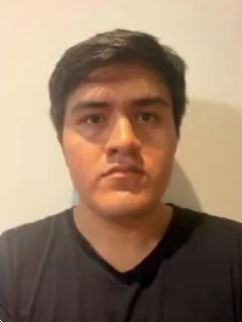
\includegraphics[height=0.34\textheight,keepaspectratio]{images/foto-original.png}\\[0.2em]
        \scriptsize Original
      \end{minipage}\hfill
      \begin{minipage}[b]{0.31\linewidth}
        \centering
        
\includegraphics[height=0.28\textheight,keepaspectratio]{images/foto-recorte.png}\\[0.2em]
        \scriptsize 512$\times$512
      \end{minipage}\hfill
      \begin{minipage}[b]{0.31\linewidth}
        \centering
        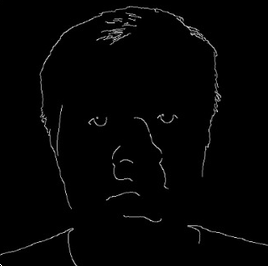
\includegraphics[height=0.28\textheight,keepaspectratio]{images/foto-canny.png}\\[0.2em]
        \scriptsize Canny
      \end{minipage}
      \vspace{0.6em}
      \begin{block}{Guía de captura}
        \scriptsize A la altura de los ojos, $\sim$1 m de distancia, de pecho hacia arriba, fondo liso y sin audífonos.
      \end{block}
    \end{column}
  \end{columns}
\end{frame}

%------------------------------------------------
% 7. Modelos generativos
\begin{frame}{Dos formas de generar sobre una GPU T4}
  \begin{columns}[T]
    \begin{column}{0.5\textwidth}
      \textbf{Dos niveles (enunciado)}
      \begin{itemize}
        \item \textbf{Intermedio:} SD 1.5 + ControlNet Canny en img2img (escala 0,85).
        \item \textbf{Básico:} SD 1.5 img2img sin ControlNet.
      \end{itemize}
      \vspace{0.25em}
      \textbf{Latencia por imagen (T4)}
      \begin{itemize}
        \item Sin LoRA: intermedio \textbf{2,61 s}, básico \textbf{1,96 s}.
        \item Con LoRA: intermedio \textbf{2,88 s}, básico \textbf{2,28 s}.
      \end{itemize}
      \vspace{0.25em}
      \scriptsize Respaldo sin GPU: filtros OpenCV (no generativo, solo continuidad de interfaz).
    \end{column}
    \begin{column}{0.48\textwidth}
      \textbf{Personalización con LoRA}
      \begin{itemize}
        \item LoRA público \texttt{detail-tweaker}, escala 0,6.
        \item \textbf{1.ª corrida (Colab):} no cargó por conflicto \texttt{torchao} (0.10) vs. \texttt{peft} ($>$0.16).
        \item \textbf{Corrección:} desinstalar \texttt{torchao}; en 2.ª corrida cargó y se aplicó a todas las variaciones.
        \item \textbf{Efecto:} +1--5\% detalle y +$\sim$0,3 s/imagen, sin cambiar la identidad.
      \end{itemize}
    \end{column}
  \end{columns}
\end{frame}

%------------------------------------------------
% 8. Interfaz
\begin{frame}{Interfaz: cada imagen espera la decisión humana}
  \begin{columns}[T]
    \begin{column}{0.5\textwidth}
      \begin{itemize}
        \item Cada variación inicia en estado \textbf{Pendiente}.
        \item Por imagen: \textbf{Aceptar/Rechazar}, calificación \textbf{1--5} y comentario.
        \item Guardado inmediato en \texttt{user\_decisions.json} (descargable) y sesión por participante.
        \item \textbf{8 estilos} agrupados en \textbf{3 paquetes}.
        \item \textbf{Prompt libre} para detalles (p. ej. color de corbata).
        \item Transparencia: se muestran recorte y bordes Canny.
      \end{itemize}
    \end{column}
    \begin{column}{0.45\textwidth}
      \centering
      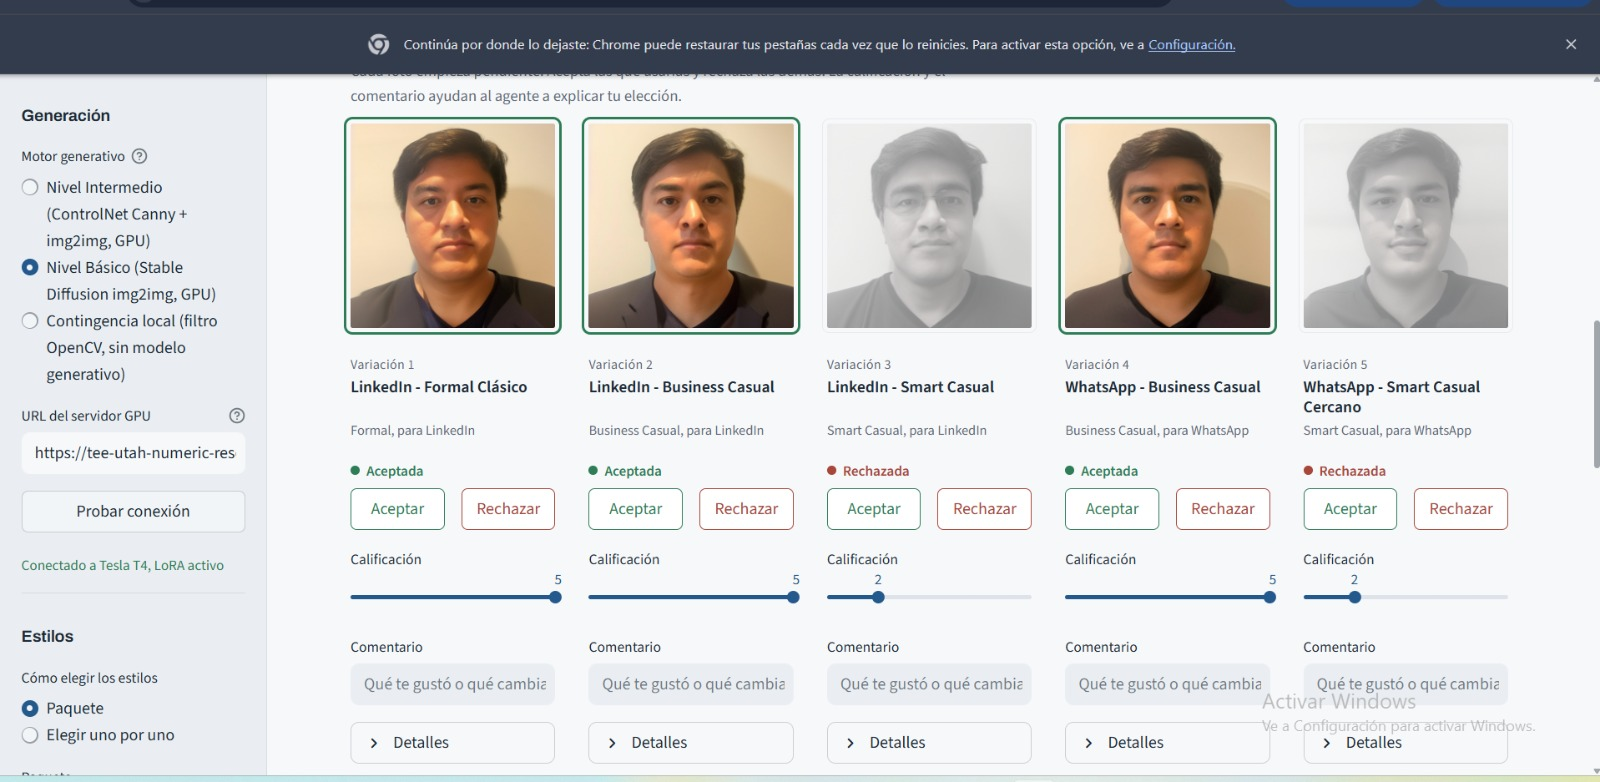
\includegraphics[width=\linewidth,height=0.66\textheight,keepaspectratio]{images/cap3.jpeg}
    \end{column}
  \end{columns}
\end{frame}

%------------------------------------------------
% 9. Demo en vivo
\begin{frame}{Demo en vivo}
  \begin{columns}[T]
    \begin{column}{0.5\textwidth}
      \textbf{Flujo de la demo}
      \begin{enumerate}
        \item Subir foto y elegir \textbf{Paquete Corporativo Multiplataforma} (5).
        \item Generar variaciones (\textbf{25--35 s} en app: 2--3 s/imagen en GPU + red).
        \item Votar las 5: Aceptar/Rechazar, calificación y comentario.
        \item Generar explicación (\textbf{Gemini}) y revisar aceptadas/rechazadas + fidelidad.
        \item Probar filtro ético: prompt \texttt{``sin ropa''} $\rightarrow$ bloqueo.
      \end{enumerate}
    \end{column}
    \begin{column}{0.48\textwidth}
      \begin{block}{Precondiciones}
        \begin{itemize}
          \item Notebook Colab (T4) ejecutado y URL \texttt{.trycloudflare.com} activa.
          \item App local conectada: \emph{Probar conexión}.
          \item \texttt{GEMINI\_API\_KEY} en \texttt{.env} (si se usa Gemini).
        \end{itemize}
      \end{block}
    \end{column}
  \end{columns}
\end{frame}

%------------------------------------------------
% 10. Resultados
\begin{frame}{Resultados: 5 variaciones por foto en segundos}
  \begin{columns}[T]
    \begin{column}{0.54\textwidth}
      \centering
      \textbf{Nivel intermedio (ControlNet Canny + img2img)}\\[0.15em]
      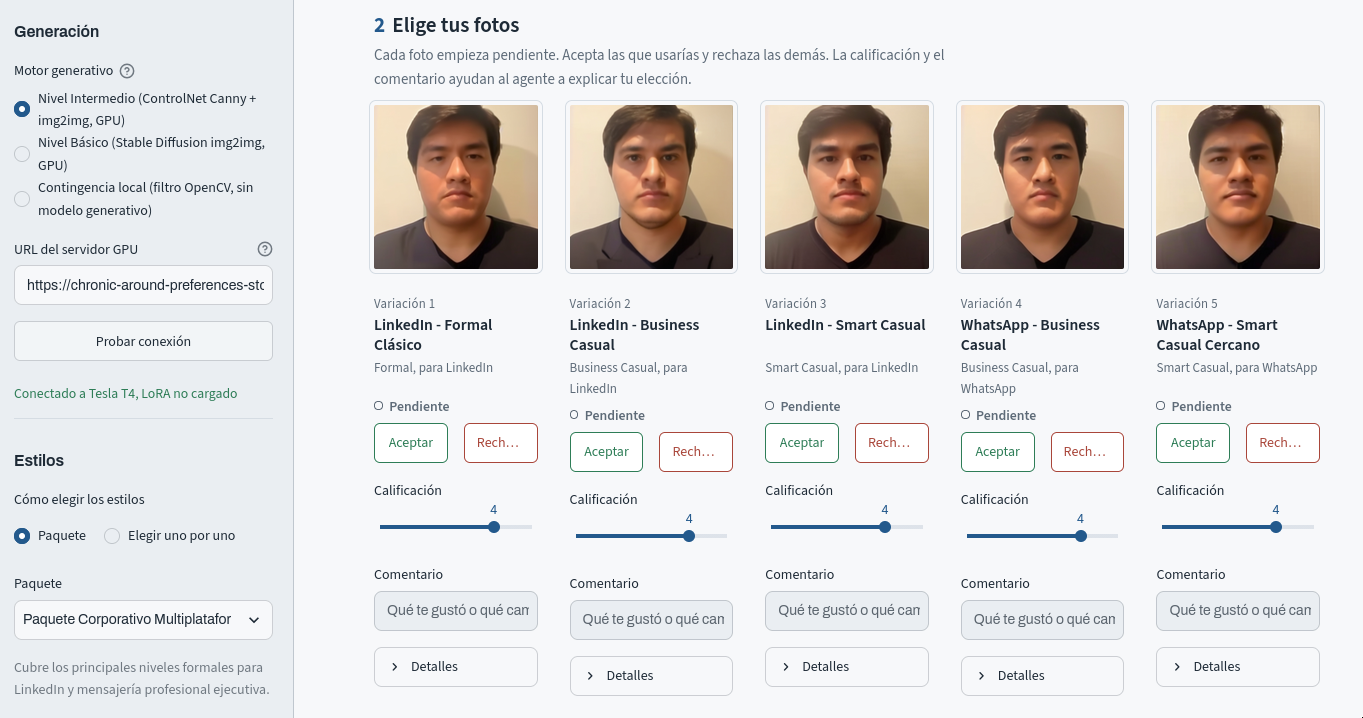
\includegraphics[width=\linewidth,height=0.24\textheight,keepaspectratio]{images/sin-lora.png}\\[0.35em]
      \textbf{Nivel básico (SD 1.5 img2img, sin ControlNet)}\\[0.15em]
      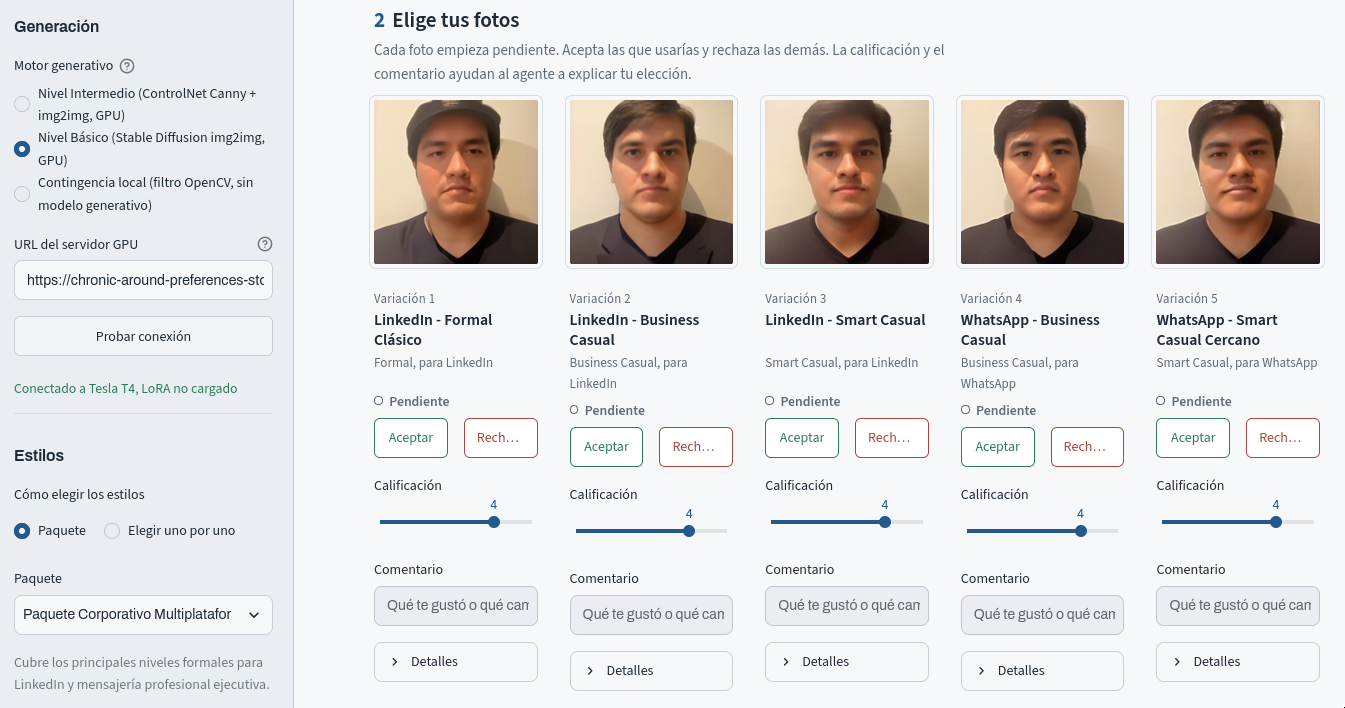
\includegraphics[width=\linewidth,height=0.24\textheight,keepaspectratio]{images/sin-lora-basico.png}
    \end{column}
    \begin{column}{0.44\textwidth}
      \textbf{Resultados reales (misma foto y semillas)}
      \begin{itemize}
        \item GPU: \textbf{2,61 s/img} (intermedio) y \textbf{1,96 s/img} (básico) sin LoRA; +$\sim$0,3 s con LoRA.
        \item App (lote de 5): \textbf{25--35 s} (5--7 s/img) incluyendo red/túnel Cloudflare.
        \item Filtro de contenido de SD: \textbf{ninguna imagen marcada}.
      \end{itemize}
    \end{column}
  \end{columns}
\end{frame}

%------------------------------------------------
% 11. Hallazgo
\begin{frame}{Hallazgo: más cambio de ropa, menos identidad}
  \begin{columns}[T]
    \begin{column}{0.6\textwidth}
      \textbf{Tensión por \emph{strength}}
      \begin{itemize}
        \item \textbf{0,42--0,48 (defecto):} ropa casi no cambia; diversidad muy baja (dif. media 0,036--0,040).
        \item \textbf{$\geq$ 0,60:} aparece el terno, pero se degrada la identidad (pelo liso $\rightarrow$ ondulado/crespo; visto en 2/5 variaciones).
        \item \textbf{Formal Clásico:} el color \emph{navy blue} se filtra al pelo.
      \end{itemize}
      \vspace{0.2em}
      \textbf{Tono de piel (medido)}
      \begin{itemize}
        \item $\Delta L^* \approx -0{,}4$ (centro de cara); hasta $-2{,}2$ (cara completa)
      \end{itemize}
    \end{column}
    \begin{column}{0.48\textwidth}
      \centering
      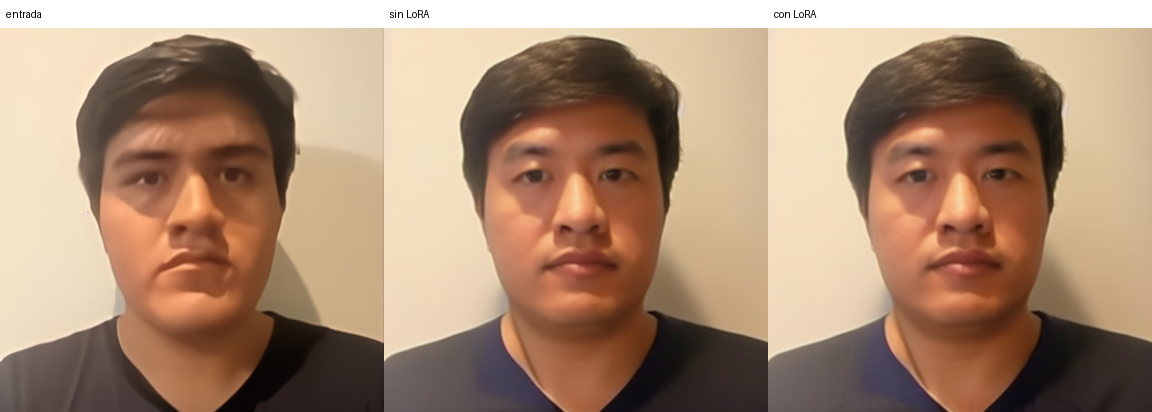
\includegraphics[width=\linewidth,height=0.34\textheight,keepaspectratio]{images/con-sin-lora.png}\\
      \scriptsize Formal Clásico, \emph{strength} 0,60: original / sin LoRA / con LoRA
      \vspace{0.35em}
      \begin{block}{Mejora propuesta}
        \textbf{Inpainting con máscara facial:} conservar píxeles de cara y pelo, y regenerar solo ropa y fondo.
      \end{block}
      \scriptsize Sesgo: el modelo empuja rasgos hacia patrones de sus datos de entrenamiento.
    \end{column}
  \end{columns}
\end{frame}

%------------------------------------------------
% 12. Agente explicador
\begin{frame}{Agente explicador: fiel a las decisiones}
  \begin{columns}[T]
    \begin{column}{0.6\textwidth}
      \textbf{Diseño y control de alucinaciones}
      \begin{itemize}
        \item Modelo principal: \textbf{Gemini 3.5 Flash Lite}; cadena de respaldo (3 modelos) y, si falla, \textbf{agente de reglas} (sin internet).
        \item La app muestra primero la \textbf{lista exacta} de aceptadas/rechazadas tomada del JSON; luego la explicación del modelo.
      \end{itemize}
      \vspace{0.25em}
      \textbf{Fidelidad medida}
      \begin{itemize}
        \item Se verifica decisión correcta por título y conteos.
        \item \textbf{10/10 corridas al 100\%} (Gemini y reglas), latencia media Gemini \textbf{11,9 s}.
      \end{itemize}
      \scriptsize Nota: versión inicial 93,8\% por falsos negativos (“no fue aceptada”); métrica corregida. Límite: asume respuesta ordenada por secciones.
    \end{column}
    \begin{column}{0.5\textwidth}
      \centering
      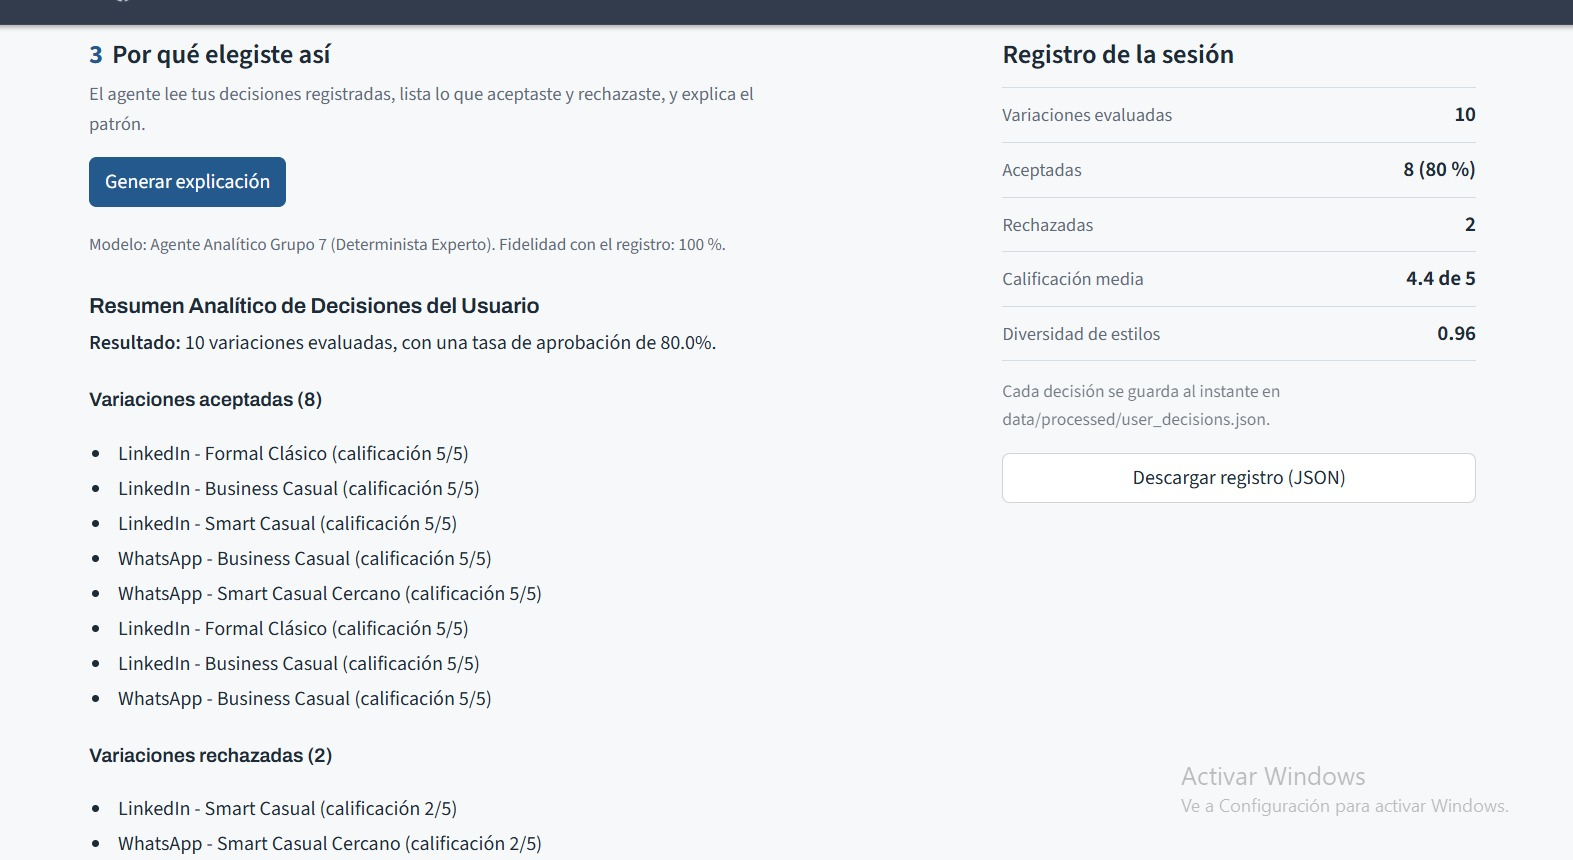
\includegraphics[width=\linewidth,height=0.64\textheight,keepaspectratio]{images/cap4.jpeg}
    \end{column}
  \end{columns}
\end{frame}

%------------------------------------------------
% 13. Ética
\begin{frame}{Ética: guardrails antes, durante y después}
  \begin{columns}[T]
    \begin{column}{0.65\textwidth}
      \textbf{Guardrails en tres momentos}
      \begin{itemize}
        \item \textbf{Antes de generar:} filtro léxico (desnudez, violencia, no profesional), normaliza tildes y números como letras (bloquea \texttt{s1n r0pa}) \emph{antes de usar la GPU}.
        \item \textbf{Al generar:} filtro de contenido de Stable Diffusion activo.
      \end{itemize}
      \vspace{0.2em}
      \textbf{Riesgos y licencias}
      \begin{itemize}
        \item Riesgos: suplantación de identidad y sesgo del modelo.
        \item SD 1.5 (CreativeML OpenRAIL-M) y ControlNet (OpenRAIL): uso con restricciones responsables.
      \end{itemize}
    \end{column}
    \begin{column}{0.45\textwidth}
      \centering
      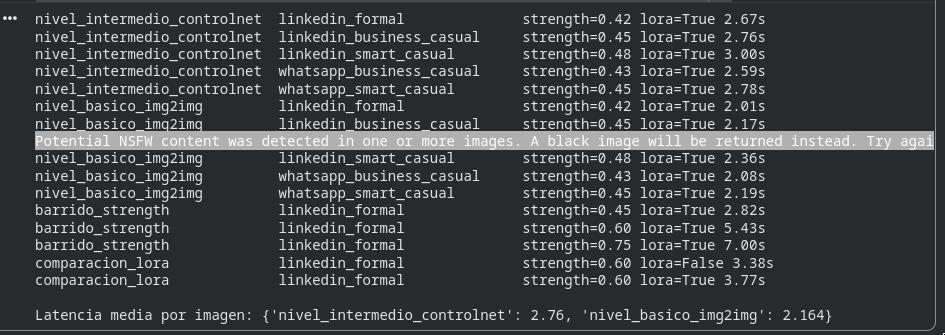
\includegraphics[width=0.92\linewidth,height=0.30\textheight,keepaspectratio]{images/etico-1.png}\\[0.25em]
      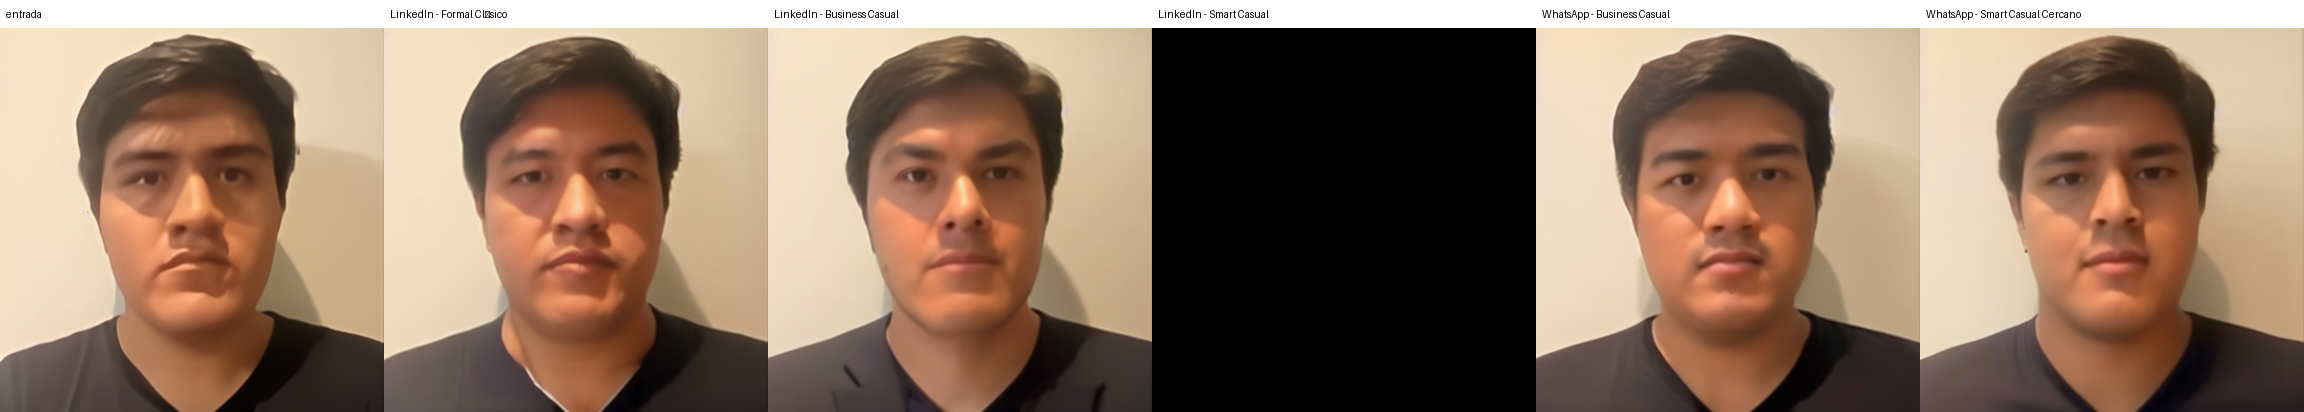
\includegraphics[width=0.92\linewidth,height=0.30\textheight,keepaspectratio]{images/etico-2.png}\\
      \scriptsize Ejemplos de bloqueo del filtro ético
    \end{column}
  \end{columns}
\end{frame}

%------------------------------------------------
% 14. Iteraciones
\begin{frame}{Iteraciones guiadas por pruebas}
  \centering
  \scriptsize
  \setlength{\tabcolsep}{5pt}
  \renewcommand{\arraystretch}{1.15}
  \begin{tabular}{@{}p{3.2cm}p{5.0cm}p{5.0cm}@{}}
    \toprule
    \textbf{Prueba} & \textbf{Problema observado} & \textbf{Cambio realizado} \\
    \midrule
    Selfie cercana / desde abajo & No detectaba cara; recorte no cabía y achataba & Reducción + ecualización, 2 clasificadores Haar, recorte siempre cuadrado \\
    Fotos de celular & Orientación incorrecta & Corrección de rotación EXIF \\
    Agente con Gemini & Modelos no disponibles/saturados (503, espera alta) & Cadena de modelos \emph{lite} + reintentos (68 s $\rightarrow$ 4--20 s) \\
    Conexión con Colab & Cortes del túnel Cloudflare & Reintento automático de petición \\
    Métrica de fidelidad & Falsos negativos con negaciones & Normalización de “no fue aceptada/rechazada” \\
    Filtro ético & Variantes como “s1n r0pa”, “shirtless” & Normalización de leetspeak y términos nuevos \\
    1.ª corrida en Colab & LoRA no cargó por conflicto con \texttt{torchao} & Desinstalar \texttt{torchao}; en 2.ª corrida el LoRA carga \\
    \bottomrule
  \end{tabular}
\end{frame}

%------------------------------------------------
% 15. Conclusiones
\begin{frame}{Conclusiones y próximos pasos}
  \begin{columns}[T]
    \begin{column}{0.54\textwidth}
      \textbf{Logros}
      \begin{itemize}
        \item Sistema completo: \textbf{2 métodos} de generación en GPU con \textbf{5 variaciones} por foto.
        \item Interfaz con decisión imagen por imagen y \textbf{registro estructurado} (JSON).
        \item Agente explicador con \textbf{100\% de fidelidad} en pruebas y guardrails éticos.
      \end{itemize}
      \vspace{0.25em}
      \textbf{Límite principal}
      \begin{itemize}
        \item En SD 1.5 img2img, cambiar la ropa y conservar la identidad están en tensión.
      \end{itemize}
    \end{column}
    \begin{column}{0.44\textwidth}
      \textbf{Próximos pasos}
      \begin{itemize}
        \item \emph{Inpainting} con máscara facial.
        \item Entrenar un LoRA propio de retrato corporativo.
        \item Evaluar la calidad de las razones del agente.
      \end{itemize}
      \vspace{0.6em}
      \begin{block}{}
        \centering
        Código en el repositorio del proyecto\\[0.4em]
        \Large \textbf{¡Gracias!}\\[0.2em]
        \normalsize Preguntas
      \end{block}
    \end{column}
  \end{columns}
\end{frame}

%------------------------------------------------
% Respaldo: Referencias
\begin{frame}[allowframebreaks]{Referencias principales (respaldo)}
  \footnotesize
  \begin{thebibliography}{99}
    \bibitem{rombach2022} Rombach, R. et al. (2022). High-resolution image synthesis with latent diffusion models. \emph{CVPR}.
    \bibitem{zhang2023} Zhang, L., Rao, A. y Agrawala, M. (2023). Adding conditional control to text-to-image diffusion models. \emph{ICCV}.
    \bibitem{hu2022} Hu, E. J. et al. (2022). LoRA: Low-rank adaptation of large language models. \emph{ICLR}.
    \bibitem{meng2022} Meng, C. et al. (2022). SDEdit: Guided image synthesis and editing with stochastic differential equations. \emph{ICLR}.
    \bibitem{lugmayr2022} Lugmayr, A. et al. (2022). RePaint: Inpainting using denoising diffusion probabilistic models. \emph{CVPR}.
    \bibitem{bianchi2023} Bianchi, F. et al. (2023). Easily accessible text-to-image generation amplifies demographic stereotypes at large scale. \emph{FAccT}.
    \bibitem{luccioni2023} Luccioni, A. S. et al. (2023). Stable bias: Evaluating societal representations in diffusion models. \emph{NeurIPS D\&B}.
    \bibitem{amershi2019} Amershi, S. et al. (2019). Guidelines for human-AI interaction. \emph{CHI}.
  \end{thebibliography}
\end{frame}

\end{document}
